\chapter{推荐系统和用户画像综述}
	\section{引言}
	自从1992年施乐的科学家为了解决信息负载的问题,第一次提出协同过滤算法,个性化推荐已经经过了二十几年的发展。1998年,林登和他的同事申请了item-to-item协同过滤技术的专利,经过多年的实践,亚马逊宣称销售的推荐占比可以占到整个销售Gross Merchandise Volume(年度成交总额)的30\%以上。随后Netflix举办的推荐算法优化竞赛,吸引了数万个团队参与角逐,期间有上百种的算法进行融合尝试,加快了推荐系统的发展,其中Sigular Value Decomposition(奇异值分解)和Gavin Potter跨界的引入心理学的方法进行建模,在诸多算法中脱颖而出。其中,矩阵分解的核心是将一个非常稀疏的用户评分矩阵R分解为两个矩阵:User特性的矩阵P和Item特性的矩阵Q,用P和Q相乘的结果R'来拟合原来的评分矩阵R,使得矩阵R'在R的非零元素那些位置上的值尽量接近R中的元素,通过定义R和R'之间的距离,把矩阵分解转化成梯度下降等求解的局部最优解问题。与此同时,Pandora、LinkedIn、Hulu、Last.fm等一些网站在个性化推荐领域都展开了不同程度的尝试,使得推荐系统在垂直领域有了不少突破性进展,但是在全品类的电商、综合的广告营销上,进展还是缓慢,仍然有很多的工作需要探索。特别是在全品类的电商中,单个模型在母婴品类的效果还比较好,但在其他品类就可能很差,很多时候需要根据品类、推荐栏位、场景等不同,设计不同的模型。同时由于用户、SKU不停地增加,需要定期对数据进行重新分析,对模型进行更新,但是定期对模型进行更新,无法保证推荐的实时性,一段时间后,由于模型训练也要相当时间,可利用传统的批处理的Hadoop的方法是无法再缩短更新频率,最终推荐效果会因为实时性问题达到一个瓶颈。推荐算法主要有基于人口统计学的推荐、基于内容的推荐、基于协同过滤的推荐等,而协同过滤算法又有基于邻域的方法、隐语义模型、基于图的随机游走算法等。基于内容的推荐解决了物品的冷启动问题,但是解决不了用户的冷启动问题,并且存在过拟合问题,即在训练集上有比较好的表现,但在实际预测中效果大打折扣,对领域知识要求也比较高,通用性和移植性比较差,换一个产品形态,往往需要重新构建一套,对于多媒体文件信息特征提取难度又比较大,往往只能通过人工标准信息。基于邻域的协同过滤算法,虽然也有冷启动问题和数据稀疏性等问题,但是没有领域知识要求,算法通用性好,增加推荐的新颖性,并且对行为丰富的物品,推荐准确度较高。基于模型的协同过滤算法在一定程度上解决了基于邻域的推荐算法面临的一些问题,在Root Mean Squared Error(均方根误差)等推荐评价指标上更优,但是通常算法复杂,计算开销大,所以目前基于邻域的协同过滤算法仍然是最为流行的推荐算法。

	\section{推荐系统的研究现状}
	Amazon的数百万图书,Netflix的10万部电影,淘宝的8亿件在线物品,以及数以亿万计用户的资料和行为记录。互联网公司最近十年的迅猛发展伴随着海量数据的积累。然而,在线用户常常面对过多的选择而显得无所适从。心理学研究证实这类情境下的用户有时做出放弃交易的决定,从而造成大量潜在的用户流失。统计技术的发展能够为在线服务商提供更有效的推荐算法,在帮助用户走出信息过载困境、改善用户体验的同时,还能够挖掘物品长尾、提升企业价值。在今天,用户不再局限于通过搜索引擎来寻找感兴趣的信息,推荐系统无所不在地为我们发现自己的潜在需求。
		\subsection{推荐系统的商业应用}
		作为全球排名第一的社交网站,Facebook就需要利用分布式推荐系统来帮助用户找到他们可能感兴趣的页面、组、事件或者游戏等。之前Facebook在其官网公布了其推荐系统的原理、性能及使用情况\citep{recmd-facebook}。目前,Facebook中推荐系统所要面对的数据集包含了约1000亿个评分、超过10亿的用户以及数百万的物品,如何在在大数据规模情况下仍然保持良好性能已经成为世界级的难题。即使是采用了分布式计算方法,Facebook仍然不可能检查每一个用户/物品对的评分。团队需要寻找更快的方法来获得每个用户排名前K的推荐物品,然后再利用推荐系统计算用户对其的评分,解决方案是采用ball tree数据结构来存储物品向量。all tree结构可以实现搜索过程10-100倍的加速,使得物品推荐工作能够在合理时间内完成。最后,Facebook给出了一些实验的结果。在2014年7月,Databricks公布了在Spark上实现ALS的性能结果。Facebook针对Amazon的数据集,基于Spark MLlib进行标准实验,与自己的旋转混合式方法的结果进行了比较。实验结果表明,Facebook的系统比标准系统要快10倍左右。而且,前者可以轻松处理超过1000亿个评分。

		目前,该方法已经用了Facebook的多个应用中,包括页面或者组的推荐等。为了能够减小系统负担,Facebook只是把度超过100的页面和组考虑为候选对象。而且,在初始迭代中,Facebook推荐系统把用户喜欢的页面/加入的组以及用户不喜欢或者拒绝加入的组都作为输入。此外,Facebook还利用基于ALS的算法,从用户获得间接的反馈。未来,Facebook会继续对推荐系统进行改进,包括利用社交图和用户连接改善推荐集合、自动化参数调整以及尝试比较好的划分机器等。Facebook推荐主页如\autoref{pic:recmd_facebook}。
		\begin{figure}
	    \centering
	      \framebox{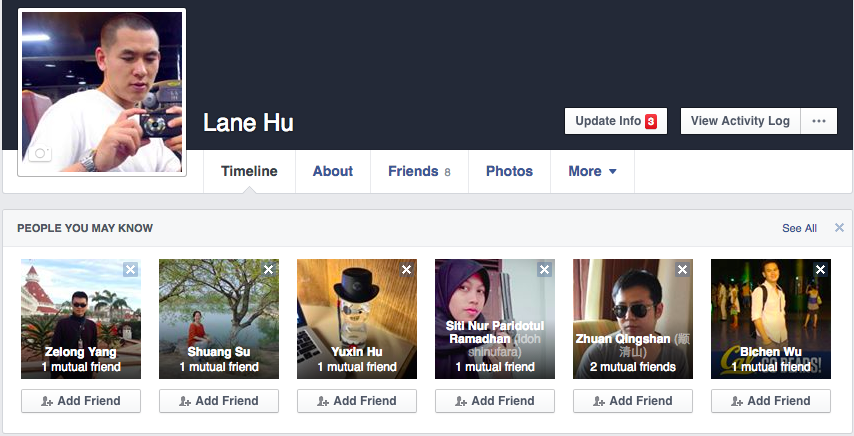
\includegraphics[scale=0.45]{figures/recmd_facebook}}
	      \figcaption{Facebook个性化推荐用户界面}
	      \label{pic:recmd_facebook}
	    \end{figure}

		豆瓣网在国内互联网行业美誉度很高,这是一家以帮助用户发现未知事物为己任的公司\citep{recmd-douban}。不用设置播放列表,也不用费心想听什么,打豆瓣电台就能收听。全新的音乐体验,让用户和喜欢的音乐不期而遇,找到符合用户口味音乐,豆瓣电台坚持这样的理念制作着全新的网络电台。通过优质的推荐系统为用户提供喜欢的音乐,在优质的电台频道下听喜欢的歌曲,豆瓣电台为喜爱音乐的人提供了这样一种全新音乐体验,音乐,本是件轻松的事,豆瓣电台做的很好。豆瓣电台的私人电台会综合用户在豆瓣上的各种音乐行为做算法推荐\citep{recmd-doubanFM}。在豆瓣音乐中,有哪些音乐标签,喜欢哪些歌手,在听哪些,想听哪些,乐评,豆列等等,即豆瓣音乐中提供的社会化网络行为,会有相关的权重算出一个公式,最开始的时候只是一个最简单的算法,在进行一段时间数据根据和用户反馈后,有了更多的权重值累加。考虑最多的是电台本身的红心、垃圾、跳过、这些用户行为数据。豆瓣电台糅合了包括算法、数据清洗与整合、音频分析技术、用户行为分析、编辑与运营、后台架构等等大量的因素,即便是推荐算法也只是算法技术中的一部分。单论推荐算法,就最简单的算法,也会极大地受到其它因素的影响,比如单曲推荐功能、新版的上线,对于算法的学习与积累都会起到极大的正面作用。简洁、小清新的界面风格,简单又易用的操作,豆瓣电台延续了豆瓣一贯的品质,豆瓣电台推荐页如\autoref{pic:recmd_doubanFM}。
		\begin{figure}
	    \centering
	      \framebox{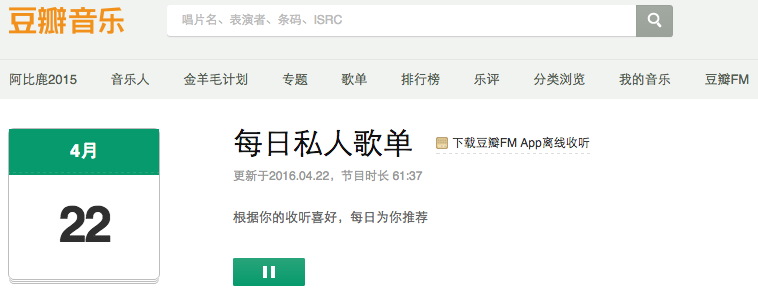
\includegraphics[scale=0.5]{figures/recmd_doubanFM}}
	      \figcaption{豆瓣电台个性化推荐用户界面}
	      \label{pic:recmd_doubanFM}
	    \end{figure}

	\subsection{推荐系统的主要方法}
	推荐系统主要是评分预测和Top-N预测,不论是哪一种推荐方式,其核心的目标是找到最适合用户c的项集合s,从集合里挑选集合是一个非常复杂的问题优化方案,通常采用的方案是用局部最优的方式,而我们只需要定义一个的效用函数,选取Top-N	\citep{recmd-Next}。
	\begin{enumerate}[(1)]
	\item 协同过滤的推荐

	推荐系统应用数据分析技术,找出用户最可能喜欢的东西推荐给用户,现在很多电子商务网站都有这个应用。目前用的比较多、比较成熟的推荐算法是协同过滤(Collaborative Filtering)推荐算法,协同过滤的基本思想是根据用户之前的喜好以及其他兴趣相近的用户的选择来给用户推荐物品。在协同过滤中,用m×n的矩阵表示用户对物品的喜好情况,一般用打分表示用户对物品的喜好程度,分数越高表示越喜欢这个物品,0表示没有买过该物品。图中行表示一个用户,列表示一个物品,$U_{ij}$表示用户i对物品j的打分情况。协同过滤分为两个过程,一个为预测过程,另一个为推荐过程。预测过程是预测用户对没有购买过的物品的可能打分值,推荐是根据预测阶段的结果推荐用户最可能喜欢的一个或Top-N个物品。协同过滤算法分为两大类,一类为基于内容的(Memory-based),一类为基于模型的(Model-based),User-based和Item-based算法均属于Memory-based类型\citep{Wikipedia},这里主要介绍User-based的协同过滤。

	有效用函数定义为用户之间的喜好上的相似性,因为基于用户的协同过滤算法是根据邻居用户的偏好信息产生对目标用户的推荐。它基于这样一个假设:如果一些用户对某一类项目的打分比较接近,则他们对其它类项目的打分也比较接近。协同过滤推荐系统采用统计计算方式搜索目标用户的相似用户,并根据相似用户对项目的打分来预测目标用户对指定项目的评分,最后选择相似度较高的前若干个相似用户的评分作为推荐结果,并反馈给用户。这种算法不仅计算简单且精确度较高,被现有的协同过滤推荐系统广泛采用。User-based协同过滤推荐算法的核心就是通过相似性度量方法计算出最近邻居集合,并将最近邻的评分结果作为推荐预测结果返回给用户。

	例如,在\autoref{tab:User-based}所示的用户一项目评分矩阵中,行代表用户,列代表项目(电影),表中的数值代表用户对某个项目的评价值。现在需要预测用户Tom对电影《枪王之王》的评分(用户Lucy对电影《阿凡达》的评分是缺失的数据)。
	由\autoref{tab:User-based}不难发现,Mary和Pete对电影的评分非常接近,Mary对《暮色3:月食》、《唐山大地震》、《阿凡达》的评分分别为3、4、4,Tom的评分分别为3、5、4,他们之间的相似度最高,因此Mary是Tom的最接近的邻居,Mary对《枪王之王》的评分结果对预测值的影响占据最大比例。相比之下,用户John和Lucy不是Tom的最近邻居,因为他们对电影的评分存在很大差距,所以JohLn和Lucy对《枪王之王》的评分对预测值的影响相对小一些。
	\begin{table}[htp]
	\centering
	\tabcaption{用户-物品表}
	\label{tab:User-based}
	\begin{tabular}{ |c|p{2cm}|p{2cm}|p{2cm}|p{2cm}| } \hline
	 & 暮色3:月食 & 唐山大地震 & 阿凡达 & 枪王之王 \\ \hline
	John & 4 & 4 & 5 & 4 \\ \hline
	Marry & 3 & 4 & 4 & 2 \\ \hline
	Lucy & 2 & 3 &  & 3 \\ \hline
	Tom & 3 & 5 & 4 &  \\ \hline
	\end{tabular}
	\end{table}

	User-based算法存在两个重大问题:1、数据稀疏性。一个大型的电子商务推荐系统一般有非常多的物品,用户可能买的其中不到1\%的物品,不同用户之间买的物品重叠性较低,导致算法无法找到一个用户的邻居,即偏好相似的用户。2、算法扩展性。最近邻居算法的计算量随着用户和物品数量的增加而增加,不适合数据量大的情况使用。 Iterm-based的基本思想是预先根据所有用户的历史偏好数据计算物品之间的相似性,然后把与用户喜欢的物品相类似的物品推荐给用户。还是以之前的例子为例,可以知道物品a和c非常相似,因为喜欢a的用户同时也喜欢c,而用户A喜欢a,所以把c推荐给用户A。因为物品直接的相似性相对比较固定,所以可以预先在线下计算好不同物品之间的相似度,把结果存在表中,当推荐时进行查表,计算用户可能的打分值,可以同时解决上面两个问题。
	\item 基于内容的推荐

	有效用函数定义为用户和物品的内容上的相似性,基于内容推荐的推荐过程:1、内容分析,从原先的物品信息(例如文档、网页、新闻、产品描述)中提取有用的信息用一种适当的方式表示。2、文件学习,作用是收集、泛化代表用户偏好的数据,生成用户概要信息。通常是采用机器学习方法从用户之前喜欢和不喜欢的物品信息中推出一个表示用户喜好的模型。例如,一个基于网页的推荐系统的属性学习器能够实现一个相关反馈的方法,将表示正面和负面例子的向量与表示用户概要信息的原型向量混合在一起。训练样例是那些附有用户正面和负面反馈信息的网页。3、过滤,通过学习用户概要信息,匹配用户概要信息和物品信息,推荐相关的物品,结果是一个二元的连续型的相关判断。后者将生成一个用户可能感兴趣的潜在物品评分列表。该匹配是计算原型向量和物品向量的余弦相似度。

	最初的基于内容的推荐是协同过滤技术的延续与发展\citep{recmd_content_based},它不需要依据用户对项目的评价意见,而是依据用户已经选择的产品内容信息计算用户之间的相似性,进而进行相应的推荐。随着机器学习等技术的完善,当前的基于内容的推荐系统可以分别对用户和产品建立配置文件,通过分析已经购买或浏览过的物品内容,建立或更新用户的配置文件。系统可以比较用户与产品配置文件之间的相似度,并直接向用户推荐与其配置文件最相似的产品——这种直接比较用户和产品相似性并进行推荐的方法,就无法纳入协同过滤的框架了。例如,在电影推荐中,基于内容的系统首先分析用户已经看过的打分比较高的电影的共性(演员、导演、语言、风格等),再推荐与这些用户感兴趣的电影内容相似度高的其它电影。基于内容的推荐算法的根本在于内容的获取和定量分析,因为在文本信息获取与过滤方面的研究较为成熟,现有很多基于内容的推荐系统都是通过分析产品的文本信息进行推荐。现在已经有一些技术可以从图片、音乐、视频中自动抽取内容信息,但是抽取后的内容多以文本、关键词(标签)、特征向量等方式表达。对这些信息的进一步处理方法,其实和文本处理是类似的。当然,文本处理发展到今天,方法已经是玲珑满目,有一部分进展我们会在下面一节中提到。本节我们介绍最为经典,也是目前应用最广泛的方法:TF-IDF方法。设有N个文本文件,关键词$k_{i}$在$n_{i}$个文件中出现,设$f_{ij}$为关键词$k_i$在文件$d_j$中出现的次数,那么$k_i$在$d_j$中的词频TF$_{ij}$定义为:TF$_{ij}$=$f_{ij}$/max$_zf_{zj}$,其中分母中的最大值是通过计算文本j中所有关键词出现的最大频率得到。附图给出了3个文本文件和5个关键词,以第一个关键词百分点为例,该关键词在文本1中出现了1次,而文本1中出现次数最多的关键词是流量,一共出现了2次,因此TF$_{11}$=0.5。一个关键词如果在许多文件中同时出现,则该关键词对于表示文件的特性贡献较小,因此要考察一个关键词i出现次数的逆,也就是$IDF_{i}$=log(N/$n_{i}$)。这个想法和我们在介绍关联规则时提到的Adamic-Adar指数思路相似。按照这个定义,对于第一个关键词百分点,IDF$_1$=log(3/2)。关键词i在文本文件j中的权重于是可以表示为$w_{ij}$=$TF_{ij}$*$IDF_{i}$,而文件j可以用一个向量$d_{j}$=($w1_{j}$,$w2_{j}$,…,$wk_{j}$),其中k是整个系统中关键词的个数。一般而言,该向量中很多元素都为0。如果把用户购买或者浏览过的产品信息抽象成一个配置文件,也用这样的向量表示出来,则可以通过直接计算没有购买过的产品相应的文件的向量和用户的配置文件的向量的相似性,把相似性最大的产品推荐给该用户。在个性化技术研究历史中非常有名的Fab系统,就是使用内容推荐的典型例子。
	\begin{lstlisting}
	文本1:不做软事,不说硬话。
	文本2:多少事,从来急;天地转,光阴迫。一万年太久,只争朝夕。
	文本3:青春之所以幸福,就因为它有前途。

	关键字包括软事、硬话、一万年、朝夕、青春、幸福、前途
	\end{lstlisting}

	总结起来,基于内容推荐的优点有:1、可以处理新用户和新产品问题。由于新用户没有选择信息,新产品没有被选信息,因此协同过滤推荐系统无法处理这类问题。但是基于内容的推荐系统可以根据用户和产品的配置文件进行相应的推荐。2、实际系统中用户对产品的打分信息非常少,协同过滤系统由于打分稀疏性的问题,受到很大的限制。基于内容的推荐系统可以不受打分稀疏性问题的约束。3、通过列出推荐项目的内容特征,可以解释为什么推荐这些产品,使用户在使用系统的时候具有很好的用户体验。与此同时,我们也注意到,基于内容的推荐系统不可避免地受到信息获取技术的约束,例如自动提取多媒体数据(图形,视频流,声音流等)的内容特征具有技术上的困难,这方面的相关应用受到了很大限制。另外,关键词的设计往往需要领域专家的参与,否则通过自动算法获得的关键词很可能没有办法表现产品特征,反而引入过度噪音。
	\end{enumerate}

	\subsection{推荐系统评测的实验方法}
	任何推荐算法都要通过评测,才能评估它的推荐质量,本节介绍评测推荐系统常用的实验方法。
		\begin{enumerate}[(1)]
		\item 离线实验,是从日志系统中取得用户的行为数据,然后将数据集分成训练数据和测试数据,比如80\%的训练数据和20\%的测试数据,然后在训练数据集上训练用户的兴趣模型,在测试集上进行测试。优点只需要一个数据集即可,不需要实际的推荐系统,离线计算,不需要人为干预,能方便快捷的测试大量不同的算法。缺点是无法获得很多实际推荐系统的指标,比如点击率、转化率等。
		\item 用户调查,离线实验往往测的最多的就是准确率,但是准确率不等于满意度,所以在算法上线之前,需要用户调查一下,测试一下用户满意度。
		\item AB测试,通过一定的规则把用户随机分成几组,并对不同组的用户采用不同的推荐算法,这样的话能够比较公平的获得不同算法在实际在线时的一些性能指标。但是缺点是周期比较长,需要长期的实验才能得到可靠的结果。
		\end{enumerate}
	\subsection{推荐系统评测的测量指标}
	推荐系统存在三个参与方:用户、物品提供者和平台。好的推荐系统总体来说是一个能令三方共赢的系统。那么如何评价推荐系统功效呢? 从用户角度,推荐系统必须满足用户的需求,给用户推荐那些令他们感兴趣的图书。推荐系统还应该能够做到准确预测用户的行为,帮助用户发现那些他们可能感兴趣但不易本发现的物品(挖掘物品的长尾)。最后推荐系统也应该能够挖掘用户潜在的兴趣,将那些与用户兴趣无关但是用户看见之后可能会感兴趣的物品推荐给用户(后文将要说明的惊喜度)。从物品提供商角度,推荐系统要让提供商的物品都能够被推荐给对其感兴趣的用户。从平台角度,推荐系统能够让本身收集到高质量的用户反馈,不断完善推荐质量,增加用户和网站的交互(用户活跃度和粘稠度?)。
		\begin{enumerate}[(1)]
		\item 用户满意度

		用户满意度是最最关键的指标,推荐系统推荐物品干嘛,就是希望推荐出来的物品能让用户满意。可以有两种方法,一是用户问卷调查,二是在线评测满意度,比如豆瓣的推荐物品旁边都有满意和不满意的按钮,亚马逊这种可以计算推荐的物品有没有被用户购买等等,一般用点击率,用户停留时间,转化率等指标来度量。
		\item 预测准确度

		如果是评分机制,则一般计算均方根误差和平均绝对误差。如果是Top-N推荐的话,则主要计算召回率和准确率。准确率就是指我推荐的n个物品中有多少个是对的,其所占的比重。召回率则是指正确结果中有多少比率的物品出现在了推荐结果中。两者的不同就是前者已推荐结果个数当除数,后者已正确结果个数当除数。
		\item 覆盖率

		就是指推荐出来的结果能不能很好的覆盖所有的物品,是不是所有的物品都有被推荐的机会。最简单的方法就是计算所有被推荐的物品占物品总数的比重,当然这个比较粗糙,更精确一点的可以信息熵和基尼系数来度量。
		\item 多样性

		推荐结果中要体现多样性,比如我看电影,我既喜欢看格斗类的电影,同时又喜欢爱装文艺,那么给我的推荐列表中就应该这两个类型的电影都有,而且得根据我爱好比例来推荐,比如我平时80\%是看格斗类的,20\%是看文艺类的,那么推荐结果中最好也是这个比例。可以根据物品间的相似度来计算,一个推荐列表中如果所有物品间的相似度都比较高,那么往往说明都是同一类物品,缺乏多样性。
		\item 新颖性

		不能说系统推荐的物品其实我都知道,那这样推荐系统就完全失去了存在的意义,一般都希望推荐一些用户不知道的物品或者没看过没买过的物品。方法一是取出已经看到过买过的物品,但这还不够,一般会计算推荐物品的平均流行度,因为通常越不热门的物品越会让用户觉得新颖。比如我爱周星驰,那么推荐《临岐》就很有新颖性,因为大家都不知道这是周星驰出演的。
		\item 惊喜度

		这个和新颖度还是有区别的,惊喜度是讲我直觉想不出来为什么会给我推荐这物品,比如电影,但是我看了之后觉得很符合我的胃口,这就是惊喜度。像上面一个例子,只要我知道是周星驰演的,那可能就没什么惊喜度,因为我知道是因为演员才给我推荐的这部电影。 注:新颖性和惊喜度暂时没有什么可以度量的标准。
		\item 信任度

		如果用户信任推荐系统,那么往往会增加与推荐系统的互动,从而获得更好的个性化推荐。增加信任的方法往往是提供推荐解释,即为什么推荐这个物品,做到有理有据。也可以通过类似facebook间的好友关系来增加信任度,一般相比于陌生人的推荐,总会选择好友给的推荐。
		\item 实时性

		新闻等一些物品具有很强的实时性,一般得在具有有效性的时候进行推荐,必须考虑推荐系统处理物品冷启动的能力。
		\end{enumerate}
	
	\section{用户画像的研究现状}
		目前基于用户画像的推荐,主要用在基于内容的推荐,从最近的RecSys大会(ACM Recommender Systems)上来看,不少公司和研究者也在尝试基于用户画像做Context-Aware的推荐。利用用户的画像,结合时间、天气等上下文信息,给用户做一些更加精准化的推荐是一个不错的方向。用户画像就是在解决把数据转化为商业价值的问题,就是从海量数据中来挖金炼银。这些高质量多维数据记录着用户长期大量的网络行为,用户画像据此来还原用户的属性特征、社会背景、兴趣喜好,甚至还能揭示内心需求、性格特点、社交人群等潜在属性。了解了用户各种消费行为和需求,精准刻画人群特征,并针对特定业务场景进行用户特征不同维度的聚合,就可以把原本冷冰冰的数据复原成栩栩如生的用户形象,从而指导和驱动业务场景和运营,发现和把握蕴藏在细分海量用户中的巨大商机。

		科学中国网曾在《大数据揭秘:淘宝上的假货、次品都卖给了谁?》中报道了淘宝不良商家如果利用买家信息欺骗消费者\citep{liar_taobao}:1、分析数据看人下刀,宰用户没商量,真相就是消费者的消费记录、购买记录、客单价等都将作为参考数据被系统识别,商家会根据这些记录评估消费者能不能分辨假货,再把假货卖给对方。2、看退货率,专欺负老实人,消费者的退货率、投诉率也会被识别到系统里,这些数据帮助商家判断用户好不好惹,退货率低于10\%的用户,会收到更多垃圾产品。3、看收货地址,决定给用户发什么货,一些淘宝店家还会根据用户收货地址所在城市,决定给用户发什么货。要是用户所在城市没有该品牌的专卖店,或者用户没有购买过该品牌的产品,那系统将会放心的把假货或者仿品发给用户。这里说明了利用用户画像可以做到精准销售,当然了,这是用户画像极其错误的用法。
	    
		\subsection{用户画像的商业应用}
		作为中国一家大型全品类综合电商,京东利用用户画像应用服务支持公司集团全业务需求\citep{user_profile_jingdong},其下游面向不同类型不同需求的人群,他们需求各不相同,从技术方案到使用方法也千差万别,因此有必要采取体系化多层次服务平台进行支持。对于公司内部,针对研发、采销、市场、客服、物流等各体系不同需求分别采取统一数据仓库、数据接口服务、产品化平台多种服务方式提供支持,针对各业务线需求场景不同,人员经验也不尽相同,用户画像的平台化给内部使用人员打造切合自身业务场景和使用经验的操作:对经验丰富的使用者提供更深入、综合参考并可自主订制或二次开发;给经验较浅的用户提供数据之外还培养其分析意识;对小白用户则可建立数据化分析运营的意识与习惯;对外部用户的支持力度也在逐步放开、加大,比如POP商家,可以满足商家针对自身店铺的个性化订制需求,并结合各种营销方式提供一站式服务解决方案。在京东用户行为日志中,每天记录着数以亿计的用户来访及海量行为。我们通过对用户行为数据进行分析和挖掘,发掘用户的偏好,逐步勾勒出用户的画像。用户画像通常通过业务经验和建立模型相结合的方法来实现,但有主次之分,有些画像更偏重于业务经验的判断,有些画像更偏重于建立模型。业务经验结合大数据分析为主勾画的人群,此类画像由于跟业务紧密相关,更多的是通过业务人员提供的经验来描述用户偏好。举个例子,比如:根据业务人员的经验,基于客户对金额、利润、信用等方面的贡献,建立多层综合指标体系,从而对用户的价值进行分级,生成用户价值的画像。一方面我们的产品经理可以根据用户价值的不同采取针对性的营销策略,另一方面通过分析我们的不同价值等级用户的占比,从而思考如何将低价值的用户发展成高价值的用户。

		再比如,通过用户在下单前的浏览情况,业务人员可以区分用户的购物性格。有些用户总是在短时间内比较了少量的商品就下单,那么他的购物性格便是冲动型;有些用户总是在反复不停的比较少量同类商品最后才下单,那么他的购物性格便是理性型;有些用户总是长时间大量的浏览了很多商品最后才下单,那么他的购物性格便是犹豫型。对于不同购物性格的用户,我们可以推荐不同类型的商品,针对冲动型用户,我们直接推荐给他/她最畅销的同类商品,而理性型用户我们推荐给他/她口碑最好的商品。并且针对每一个用户,我们根据其购物性格定制了个性化的营销手段。

		以建立模型为主勾画的人群,我们不能认为买过母婴类用品的用户家里就一定有小孩,因为这次购买很有可能是替别人代买或者送礼物。所以我们要判断这个用户所购买的母婴类商品是否是给自己买。根据用户下单前浏览情况、收货地址、对商品的评价等多种信息建立模型,最终判断出用户家庭是否有小孩。再根据购买的商品标签,比如奶粉的段数,童书适应年龄段等信息,建立孩子成长模型,在孩子所处不同的阶段进行精准营销。

		京东拥有最全的品类,各品类间用户转化成为我们业务的一个重点。挖掘一个品类的潜在用户,首先要找出此品类已有的用户,然后通过这些用户的行为、偏好、画像等信息对用户细分,挖掘其独有的特征,最后通过这些特征建立模型定位出该品类的潜在用户。

		这一阶段主要是为了验证我们为用户描绘的画像是否准确。比如一个用户的画像是:性别男、年龄在36岁~45岁之间、家里有小孩、未婚、有车一族、购买等级高。我们可以很快发现家里有小孩且未婚这一矛盾的结果。首先,我们可以判断对这个用户的画像肯定有问题的。接下来我们看这个用户的画像,似乎只有未婚这一条与其他画像格格不入。通过模型之间的验证,我们发现一些错误案例并分析原因,进而改进我们的模型。

		2014年的618前夕京东范产品的数据接口服务,将用户画像模型充分应用到产品当中,根据族群的差异化特征,帮助业务部门找到营销机会、运营方向,全面提高产品的核心影响力,增强产品用户体验。应用模型包括:年龄、性格、购物偏好、购买力等用户特征,诠释勾勒出用户在京东上的体貌特征,赋予一定的潮流“范儿”的概念,贴近用户。

		京东数聚汇也是用户画像的一个典型应用,通过深度分析年度网购用户的行为,挖掘网络购物趣味数据,结合用户画像,从用户的购物行为入手,结合年度流行热点,分析不同地域网购人群的购物习惯和喜好,为网民展现一场京东大数据的饕餮盛宴,同时给商家和消费者提供了经营和购物参考。

		\subsection{用户画像的组成部分}
		基于内容和用户画像的个性化推荐,有两个实体:内容和用户。需要有一个联系这两者的东西,即为标签。内容转换为标签即为内容特征化,用户则称为用户特征化。因此,对于基于用户画像的推荐,主要分为以下几个关键部分:
		\begin{enumerate}[(1)]
		\item 标签库

		标签是联系用户与物品、内容以及物品、内容之间的纽带,也是反应用户兴趣的重要数据源。标签库的最终用途在于对用户进行行为、属性标记。是将其他实体转换为计算机可以理解的语言关键的一步。标签库则是对标签进行聚合的系统,包括对标签的管理、更新等。在用户画像的过程中有一个很重要的概念叫做颗粒度,就是我们的用户画像应该细化到哪种程度。举一个极端的例子,如果“用户画像”最细的颗粒度应该是细到每一个用户每一具体的生活场景中,但是这基本上是一个不可能完成的任务,同时如果用户画像的颗粒度太大,对于产品设计的指导意义又相对变小了,所以把握好画像的总体丰富程度显得异常重要了。可通过调查问卷的形式来减小颗粒度。一般来说,标签是以层级的形式组织的。可以有一级维度、二级维度等。标签的来源主要有:已有内容的标签。网络抓取流行标签。对运营的内容进行关键词提取,对于内容的关键词提取,使用结巴分词和TFIDF即可。
		\item 内容特征化

		内容特征化即给内容打标签。目前有两种方式:人工打标签和机器自动打标签。针对机器自动打标签,需要采取机器学习的相关算法来实现,即针对一系列给定的标签,给内容选取其中匹配度最高的几个标签。这不同于通常的分类和聚类算法。可以采取使用分词 + Word2Vec来实现,过程:将文本语料进行分词,以空格,tab隔开都可以,使用结巴分词。使用word2vec训练词的相似度模型。使用tfidf提取内容的关键词A,B,C。遍历每一个标签,计算关键词与此标签的相似度之和。取出TopN相似度最高的标签即为此内容的标签。
		\item 用户特征化

		用户特征化即为用户打标签。通过用户的行为日志和一定的模型算法得到用户的每个标签的权重。用户对内容的行为:点赞、不感兴趣、点击、浏览。对用户的反馈行为如点赞赋予权值1,不感兴趣赋予-1;对于用户的浏览行为,则可使用点击/浏览作为权值。对内容发生的行为可以认为对此内容所带的标签的行为。用户的兴趣是时间衰减的,即离当前时间越远的兴趣比重越低。时间衰减函数使用1/[log(t)+1], t为事件发生的时间距离当前时间的大小。要考虑到热门内容会干预用户的标签,需要对热门内容进行降权。使用click/pv作为用户浏览行为权值即可达到此目的。此外,还需要考虑噪声的干扰,如标题党等。
		\item 隐语义推荐

		有了内容特征和用户特征,可以使用隐语义模型进行推荐。这里可以使用其简化形式,以达到实时计算的目的。用户对于某一个内容的兴趣度(可以认为是CTR):
	    \begin{equation}
	    r_{uc}=q_c \ast \sum_{i=1}^{n} m_{ci} \ast n_{ui}
	    \label{CTR}
	    \end{equation}
	    其中i=1…N是内容c具有的标签,m$_{ci}$指的内容c和标签i的关联度(默认为是1),n$_{ui}$指的是用户u的标签i的权重值,当用户不具有此标签时n$_{ui}$=0,q指的是内容c的质量,可以使用点击率(click/page view)表示。

		\end{enumerate}
		\subsection{用户画像的构建周期}
		用户画像,即用户信息标签化,就是企业通过收集与分析消费者社会属性、生活习惯、消费行为等主要信息的数据之后,完美地抽象出一个用户的商业全貌作是企业应用大数据技术的基本方式。构建周期如\autoref{pic:userprofile_process}。
		\begin{figure}
	    \centering
	      \framebox{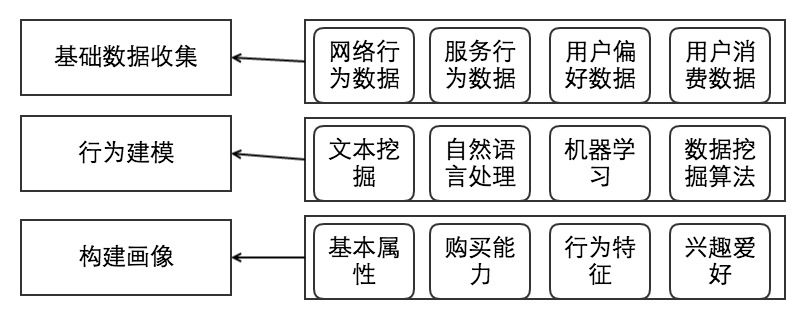
\includegraphics[scale=0.45]{figures/userprofile_process}}
	      \figcaption{用户画像的构建周期示意图}
	      \label{pic:userprofile_process}
	    \end{figure}
	    \begin{enumerate}[(1)]
	    \item 数据收集

	    数据收集大致分为网络行为数据、服务内行为数据、用户内容偏好数据、用户交易数据这四类。网络行为数据:活跃人数、页面浏览量、访问时长、激活率、外部触点、社交数据等。服务内行为数据:浏览路径、页面停留时间、访问深度、唯一页面浏览次数等。用户内容便好数据:浏览/收藏内容、评论内容、互动内容、生活形态偏好、品牌偏好等。用户交易数据(交易类服务):贡献率、客单价、连带率、回头率、流失率等。收集到的数据不会是100\%准确的,都具有不确定性,这就需要在后面的阶段中建模来再判断,比如某用户在性别一栏填的男,但通过其行为偏好可判断其性别为女的概率更大。
	    \item 行为建模

	    该阶段是对上阶段收集到数据的处理,进行行为建模,以抽象出用户的标签,这个阶段注重的应是大概率事件,通过数学算法模型尽可能地排除用户的偶然行为。这时也要用到机器学习,对用户的行为、偏好进行猜测,好比一个 y=kx+b 的算法,X 代表已知信息,Y 是用户偏好,通过不断的精确k和b来精确Y。在这个阶段,需要用到很多模型来给用户贴标签。
	    \item 用户画像基本成型

	    该阶段可以说是二阶段的一个深入,要把用户的基本属性(年龄、性别、地域)、购买能力、行为特征、兴趣爱好、心理特征、社交网络大致地标签化。因为用户画像永远也无法100%地描述一个人,只能做到不断地去逼近一个人,因此,用户画像既应根据变化的基础数据不断修正,又要根据已知数据来抽象出新的标签使用户画像越来越立体。
	    \item 数据可视化

	    最后是数据可视化分析,这是把用户画像真正利用起来的一步,在此步骤中一般是针对群体的分析,比如可以根据用户价值来细分出核心用户、评估某一群体的潜在价值空间,以作出针对性的运营。典型的用户画像如\autoref{pic:user_profile}
	    \end{enumerate}
		\begin{figure}
	    \centering
	      \framebox{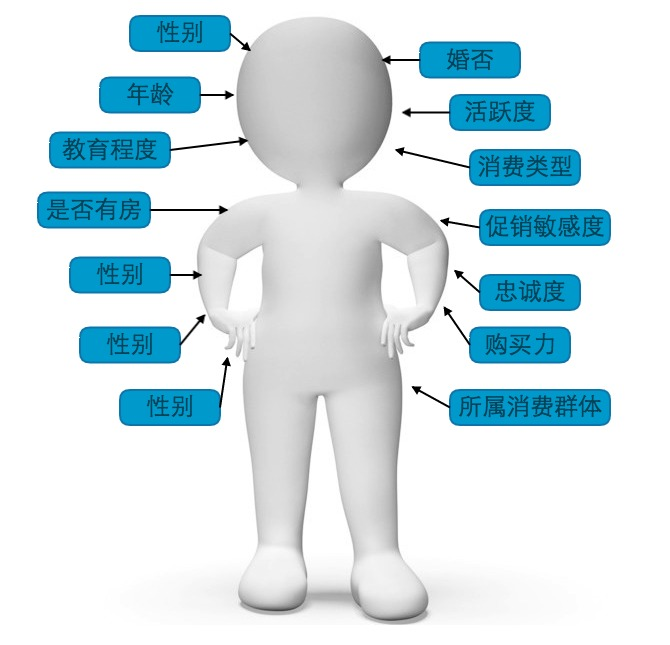
\includegraphics[scale=0.4]{figures/user_profile}}
	      \figcaption{用户画像示意图}
	      \label{pic:user_profile}
	    \end{figure}

	\section{本章小结}
	本章简单概述了推荐系统的主要任务和问题。从商业应用和学术研究两个角度介绍了推荐系统研究的现状,并讨论了推荐系统的主要评测指标。然后介绍了用户画像的研究现状,讨论了相关的建模过程。